%TODO: the fact that we we do not use tree structure violates "the lore". I have never seen AHP algorithms that would be
%implemented in this way.

%TODO: MAYBE: I have managed to formulate formal requirements for the graph that we use. What
%if I write them as well? I define there a notion of level (to some extent), and reveal constraints that make the
%recursive approach applicable.

%TODO: Constraints. We do not:
% 1. Delve into an agent's reasoning process;
% 2. Imply any particular structure of the graph;
% 3. Imply any particular implementation of an agent, neither its reasoning process (although we model that in our
%    "implementation" section)

% TODO: plan
% -- hierarchy of preferences
% -- formal description of the graph. Definitions: levels
% -- separation of responsibilities, the actual approach to simulation
% -- definitions: aspects, contexts
% -- fusion of tactical decisions up to the general objective (moving up the contexts)
% -- using AHP for this
% -- the recursive algorithm implementing the idea

In order to incorporate both strategic and tactical objectives into the decision making process we propose to represent
the latter as a result of decomposing strategic ones. By that, we do not necessarily mean that tactical objectives have
to be mutually exclusive components, represent dependencies or certain milestones, although that is definitely an
option. It implies that any lower-level objective may be a part of two or more higher-level ones. This decomposition can
be represented as a hierarchy or preferences or preference graph (Figure \ref{fig:prefgraph-concept}).
%TODO: ref figure

\begin{figure}[hbt!]
    \centering
    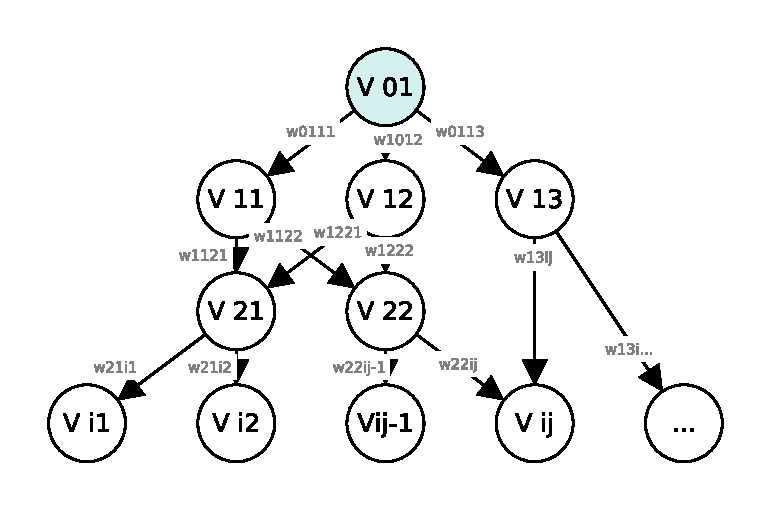
\includegraphics[width=0.7\textwidth]{prefgraph-concept.eps}

    \caption{\small An example of a preference graph}
    \label{fig:prefgraph-concept}
\end{figure}

To enrich
the semantics of the decomposition process, we propose to not to limit it by just one iteration.
